\documentclass{standalone}
\usepackage{tikz}
\usetikzlibrary{patterns, positioning}


\begin{document}
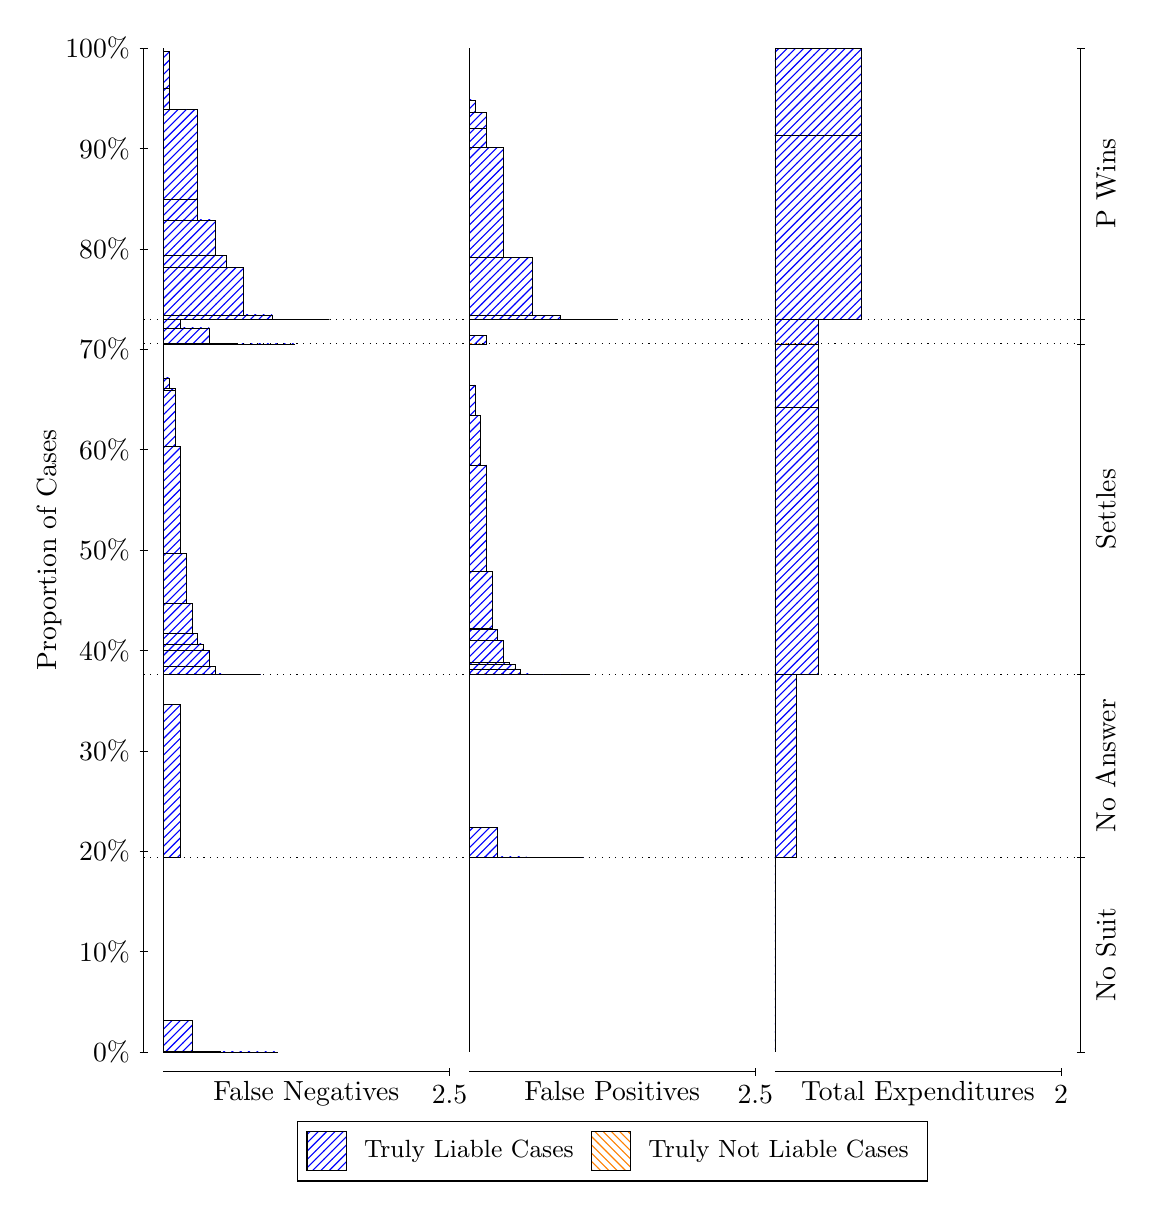
\begin{tikzpicture}
\draw[black, very thin] (1.5,1.75) -- (1.5,14.5);
\node[rotate=90, text=black, anchor=center] at (0.3, 8.125) {Proportion of Cases};
\draw[black, very thin] (1.45,1.75) -- (1.55,1.75);
\node[text=black, anchor=east] at (1.45, 1.75) {0\%};
\draw[black, very thin] (1.45,3.025) -- (1.55,3.025);
\node[text=black, anchor=east] at (1.45, 3.025) {10\%};
\draw[black, very thin] (1.45,4.3) -- (1.55,4.3);
\node[text=black, anchor=east] at (1.45, 4.3) {20\%};
\draw[black, very thin] (1.45,5.575) -- (1.55,5.575);
\node[text=black, anchor=east] at (1.45, 5.575) {30\%};
\draw[black, very thin] (1.45,6.85) -- (1.55,6.85);
\node[text=black, anchor=east] at (1.45, 6.85) {40\%};
\draw[black, very thin] (1.45,8.125) -- (1.55,8.125);
\node[text=black, anchor=east] at (1.45, 8.125) {50\%};
\draw[black, very thin] (1.45,9.4) -- (1.55,9.4);
\node[text=black, anchor=east] at (1.45, 9.4) {60\%};
\draw[black, very thin] (1.45,10.675) -- (1.55,10.675);
\node[text=black, anchor=east] at (1.45, 10.675) {70\%};
\draw[black, very thin] (1.45,11.95) -- (1.55,11.95);
\node[text=black, anchor=east] at (1.45, 11.95) {80\%};
\draw[black, very thin] (1.45,13.225) -- (1.55,13.225);
\node[text=black, anchor=east] at (1.45, 13.225) {90\%};
\draw[black, very thin] (1.45,14.5) -- (1.55,14.5);
\node[text=black, anchor=east] at (1.45, 14.5) {100\%};

\draw[black, very thin] (13.4,1.75) -- (13.4,14.5);
\draw[black, very thin] (13.35,1.75) -- (13.45,1.75);
\node[anchor=west] at (13.35, 1.75) {};
\draw[black, very thin] (13.35,4.2243) -- (13.45,4.2243);
\node[anchor=west] at (13.35, 4.2243) {};
\draw[black, very thin] (13.35,6.5495) -- (13.45,6.5495);
\node[anchor=west] at (13.35, 6.5495) {};
\draw[black, very thin] (13.35,10.742) -- (13.45,10.742);
\node[anchor=west] at (13.35, 10.742) {};
\draw[black, very thin] (13.35,11.056) -- (13.45,11.056);
\node[anchor=west] at (13.35, 11.056) {};
\draw[black, very thin] (13.35,14.5) -- (13.45,14.5);
\node[anchor=west] at (13.35, 14.5) {};

\draw[black, very thin, pattern color=blue, pattern=north east lines] (1.75,1.75) rectangle (3.2033,1.75);
\draw[black, very thin, pattern color=blue, pattern=north east lines] (1.75,1.75) rectangle (2.84,1.75);
\draw[black, very thin, pattern color=blue, pattern=north east lines] (1.75,1.75) rectangle (2.4767,1.7535);
\draw[black, very thin, pattern color=blue, pattern=north east lines] (1.75,1.7535) rectangle (2.1133,2.1551);
\draw[black, very thin, pattern color=orange, pattern=north west lines] (1.75,2.1551) rectangle (1.75,2.1551);
\draw[black, very thin, pattern color=blue, pattern=north east lines] (1.75,2.1551) rectangle (1.75,4.2243);
\draw[black, very thin, pattern color=blue, pattern=north east lines] (1.75,4.2243) rectangle (1.968,6.1688);
\draw[black, very thin, pattern color=orange, pattern=north west lines] (1.75,6.1688) rectangle (1.75,6.1688);
\draw[black, very thin, pattern color=blue, pattern=north east lines] (1.75,6.1688) rectangle (1.75,6.5495);
\draw[black, very thin, pattern color=blue, pattern=north east lines] (1.75,6.5495) rectangle (2.9853,6.5495);
\draw[black, very thin, pattern color=blue, pattern=north east lines] (1.75,6.5495) rectangle (2.84,6.5495);
\draw[black, very thin, pattern color=blue, pattern=north east lines] (1.75,6.5495) rectangle (2.6947,6.5499);
\draw[black, very thin, pattern color=blue, pattern=north east lines] (1.75,6.5499) rectangle (2.622,6.5499);
\draw[black, very thin, pattern color=blue, pattern=north east lines] (1.75,6.5499) rectangle (2.5493,6.5503);
\draw[black, very thin, pattern color=blue, pattern=north east lines] (1.75,6.5503) rectangle (2.4767,6.552);
\draw[black, very thin, pattern color=blue, pattern=north east lines] (1.75,6.552) rectangle (2.404,6.6449);
\draw[black, very thin, pattern color=blue, pattern=north east lines] (1.75,6.6449) rectangle (2.3313,6.8467);
\draw[black, very thin, pattern color=blue, pattern=north east lines] (1.75,6.8467) rectangle (2.2587,6.933);
\draw[black, very thin, pattern color=blue, pattern=north east lines] (1.75,6.933) rectangle (2.186,7.0703);
\draw[black, very thin, pattern color=blue, pattern=north east lines] (1.75,7.0703) rectangle (2.1133,7.4516);
\draw[black, very thin, pattern color=blue, pattern=north east lines] (1.75,7.4516) rectangle (2.0407,8.0855);
\draw[black, very thin, pattern color=blue, pattern=north east lines] (1.75,8.0855) rectangle (1.968,9.4424);
\draw[black, very thin, pattern color=blue, pattern=north east lines] (1.75,9.4424) rectangle (1.8953,10.158);
\draw[black, very thin, pattern color=blue, pattern=north east lines] (1.75,10.158) rectangle (1.8953,10.175);
\draw[black, very thin, pattern color=blue, pattern=north east lines] (1.75,10.175) rectangle (1.8227,10.312);
\draw[black, very thin, pattern color=orange, pattern=north west lines] (1.75,10.312) rectangle (1.75,10.312);
\draw[black, very thin, pattern color=blue, pattern=north east lines] (1.75,10.312) rectangle (1.75,10.742);
\draw[black, very thin, pattern color=blue, pattern=north east lines] (1.75,10.742) rectangle (3.4213,10.742);
\draw[black, very thin, pattern color=blue, pattern=north east lines] (1.75,10.742) rectangle (3.058,10.742);
\draw[black, very thin, pattern color=blue, pattern=north east lines] (1.75,10.742) rectangle (2.6947,10.748);
\draw[black, very thin, pattern color=blue, pattern=north east lines] (1.75,10.748) rectangle (2.3313,10.945);
\draw[black, very thin, pattern color=blue, pattern=north east lines] (1.75,10.945) rectangle (1.968,11.056);
\draw[black, very thin, pattern color=orange, pattern=north west lines] (1.75,11.056) rectangle (1.75,11.056);
\draw[black, very thin, pattern color=blue, pattern=north east lines] (1.75,11.056) rectangle (3.8573,11.056);
\draw[black, very thin, pattern color=blue, pattern=north east lines] (1.75,11.056) rectangle (3.494,11.057);
\draw[black, very thin, pattern color=blue, pattern=north east lines] (1.75,11.057) rectangle (3.276,11.057);
\draw[black, very thin, pattern color=blue, pattern=north east lines] (1.75,11.057) rectangle (3.1307,11.11);
\draw[black, very thin, pattern color=blue, pattern=north east lines] (1.75,11.11) rectangle (2.9127,11.11);
\draw[black, very thin, pattern color=blue, pattern=north east lines] (1.75,11.11) rectangle (2.7673,11.714);
\draw[black, very thin, pattern color=blue, pattern=north east lines] (1.75,11.714) rectangle (2.5493,11.87);
\draw[black, very thin, pattern color=blue, pattern=north east lines] (1.75,11.87) rectangle (2.404,12.317);
\draw[black, very thin, pattern color=blue, pattern=north east lines] (1.75,12.317) rectangle (2.186,12.573);
\draw[black, very thin, pattern color=blue, pattern=north east lines] (1.75,12.573) rectangle (2.186,13.717);
\draw[black, very thin, pattern color=blue, pattern=north east lines] (1.75,13.717) rectangle (2.0407,13.717);
\draw[black, very thin, pattern color=blue, pattern=north east lines] (1.75,13.717) rectangle (1.8227,13.994);
\draw[black, very thin, pattern color=blue, pattern=north east lines] (1.75,13.994) rectangle (1.8227,14.455);
\draw[black, very thin, pattern color=orange, pattern=north west lines] (1.75,14.455) rectangle (1.75,14.455);
\draw[black, very thin, pattern color=blue, pattern=north east lines] (1.75,14.455) rectangle (1.75,14.5);
\draw[black, very thin, pattern color=orange, pattern=north west lines] (5.6333,1.75) rectangle (5.6333,1.75);
\draw[black, very thin, pattern color=blue, pattern=north east lines] (5.6333,1.75) rectangle (5.6333,4.2243);
\draw[black, very thin, pattern color=orange, pattern=north west lines] (5.6333,4.2243) rectangle (7.0867,4.2243);
\draw[black, very thin, pattern color=blue, pattern=north east lines] (5.6333,4.2243) rectangle (7.0867,4.2243);
\draw[black, very thin, pattern color=blue, pattern=north east lines] (5.6333,4.2243) rectangle (6.7233,4.2243);
\draw[black, very thin, pattern color=blue, pattern=north east lines] (5.6333,4.2243) rectangle (6.36,4.2275);
\draw[black, very thin, pattern color=blue, pattern=north east lines] (5.6333,4.2275) rectangle (5.9967,4.605);
\draw[black, very thin, pattern color=blue, pattern=north east lines] (5.6333,4.605) rectangle (5.6333,6.5495);
\draw[black, very thin, pattern color=orange, pattern=north west lines] (5.6333,6.5495) rectangle (7.1593,6.5495);
\draw[black, very thin, pattern color=blue, pattern=north east lines] (5.6333,6.5495) rectangle (7.1593,6.5495);
\draw[black, very thin, pattern color=orange, pattern=north west lines] (5.6333,6.5495) rectangle (7.014,6.5495);
\draw[black, very thin, pattern color=blue, pattern=north east lines] (5.6333,6.5495) rectangle (7.014,6.5495);
\draw[black, very thin, pattern color=orange, pattern=north west lines] (5.6333,6.5495) rectangle (6.8687,6.5495);
\draw[black, very thin, pattern color=blue, pattern=north east lines] (5.6333,6.5495) rectangle (6.8687,6.5495);
\draw[black, very thin, pattern color=blue, pattern=north east lines] (5.6333,6.5495) rectangle (6.796,6.5495);
\draw[black, very thin, pattern color=orange, pattern=north west lines] (5.6333,6.5495) rectangle (6.7233,6.5495);
\draw[black, very thin, pattern color=blue, pattern=north east lines] (5.6333,6.5495) rectangle (6.7233,6.5495);
\draw[black, very thin, pattern color=blue, pattern=north east lines] (5.6333,6.5495) rectangle (6.6507,6.5495);
\draw[black, very thin, pattern color=orange, pattern=north west lines] (5.6333,6.5495) rectangle (6.578,6.5495);
\draw[black, very thin, pattern color=blue, pattern=north east lines] (5.6333,6.5495) rectangle (6.578,6.5495);
\draw[black, very thin, pattern color=blue, pattern=north east lines] (5.6333,6.5495) rectangle (6.5053,6.5495);
\draw[black, very thin, pattern color=orange, pattern=north west lines] (5.6333,6.5495) rectangle (6.4327,6.5495);
\draw[black, very thin, pattern color=blue, pattern=north east lines] (5.6333,6.5495) rectangle (6.4327,6.5503);
\draw[black, very thin, pattern color=blue, pattern=north east lines] (5.6333,6.5503) rectangle (6.36,6.5506);
\draw[black, very thin, pattern color=blue, pattern=north east lines] (5.6333,6.5506) rectangle (6.2873,6.5506);
\draw[black, very thin, pattern color=orange, pattern=north west lines] (5.6333,6.5506) rectangle (6.2873,6.5506);
\draw[black, very thin, pattern color=blue, pattern=north east lines] (5.6333,6.5506) rectangle (6.2873,6.6041);
\draw[black, very thin, pattern color=blue, pattern=north east lines] (5.6333,6.6041) rectangle (6.2147,6.6688);
\draw[black, very thin, pattern color=blue, pattern=north east lines] (5.6333,6.6688) rectangle (6.142,6.7006);
\draw[black, very thin, pattern color=blue, pattern=north east lines] (5.6333,6.7006) rectangle (6.0693,6.9792);
\draw[black, very thin, pattern color=blue, pattern=north east lines] (5.6333,6.9792) rectangle (5.9967,7.1161);
\draw[black, very thin, pattern color=blue, pattern=north east lines] (5.6333,7.1161) rectangle (5.924,7.1336);
\draw[black, very thin, pattern color=blue, pattern=north east lines] (5.6333,7.1336) rectangle (5.924,7.8487);
\draw[black, very thin, pattern color=blue, pattern=north east lines] (5.6333,7.8487) rectangle (5.8513,9.2056);
\draw[black, very thin, pattern color=blue, pattern=north east lines] (5.6333,9.2056) rectangle (5.7787,9.8395);
\draw[black, very thin, pattern color=blue, pattern=north east lines] (5.6333,9.8395) rectangle (5.706,10.221);
\draw[black, very thin, pattern color=blue, pattern=north east lines] (5.6333,10.221) rectangle (5.6333,10.742);
\draw[black, very thin, pattern color=orange, pattern=north west lines] (5.6333,10.742) rectangle (5.8513,10.742);
\draw[black, very thin, pattern color=blue, pattern=north east lines] (5.6333,10.742) rectangle (5.8513,10.852);
\draw[black, very thin, pattern color=blue, pattern=north east lines] (5.6333,10.852) rectangle (5.6333,11.056);
\draw[black, very thin, pattern color=orange, pattern=north west lines] (5.6333,11.056) rectangle (7.5227,11.056);
\draw[black, very thin, pattern color=blue, pattern=north east lines] (5.6333,11.056) rectangle (7.5227,11.056);
\draw[black, very thin, pattern color=orange, pattern=north west lines] (5.6333,11.056) rectangle (7.1593,11.056);
\draw[black, very thin, pattern color=blue, pattern=north east lines] (5.6333,11.056) rectangle (7.1593,11.057);
\draw[black, very thin, pattern color=orange, pattern=north west lines] (5.6333,11.057) rectangle (6.796,11.057);
\draw[black, very thin, pattern color=blue, pattern=north east lines] (5.6333,11.057) rectangle (6.796,11.102);
\draw[black, very thin, pattern color=orange, pattern=north west lines] (5.6333,11.102) rectangle (6.578,11.102);
\draw[black, very thin, pattern color=blue, pattern=north east lines] (5.6333,11.102) rectangle (6.578,11.102);
\draw[black, very thin, pattern color=orange, pattern=north west lines] (5.6333,11.102) rectangle (6.4327,11.102);
\draw[black, very thin, pattern color=blue, pattern=north east lines] (5.6333,11.102) rectangle (6.4327,11.839);
\draw[black, very thin, pattern color=orange, pattern=north west lines] (5.6333,11.839) rectangle (6.2147,11.839);
\draw[black, very thin, pattern color=blue, pattern=north east lines] (5.6333,11.839) rectangle (6.2147,11.84);
\draw[black, very thin, pattern color=blue, pattern=north east lines] (5.6333,11.84) rectangle (6.0693,13.24);
\draw[black, very thin, pattern color=blue, pattern=north east lines] (5.6333,13.24) rectangle (5.8513,13.477);
\draw[black, very thin, pattern color=orange, pattern=north west lines] (5.6333,13.477) rectangle (5.8513,13.477);
\draw[black, very thin, pattern color=blue, pattern=north east lines] (5.6333,13.477) rectangle (5.8513,13.686);
\draw[black, very thin, pattern color=blue, pattern=north east lines] (5.6333,13.686) rectangle (5.706,13.842);
\draw[black, very thin, pattern color=blue, pattern=north east lines] (5.6333,13.842) rectangle (5.6333,14.5);
\draw[black, very thin, pattern color=orange, pattern=north west lines] (9.5167,1.75) rectangle (9.5167,1.75);
\draw[black, very thin, pattern color=blue, pattern=north east lines] (9.5167,1.75) rectangle (9.5167,4.2243);
\draw[black, very thin, pattern color=orange, pattern=north west lines] (9.5167,4.2243) rectangle (9.7892,4.2243);
\draw[black, very thin, pattern color=blue, pattern=north east lines] (9.5167,4.2243) rectangle (9.7892,6.5495);
\draw[black, very thin, pattern color=orange, pattern=north west lines] (9.5167,6.5495) rectangle (10.062,6.5495);
\draw[black, very thin, pattern color=blue, pattern=north east lines] (9.5167,6.5495) rectangle (10.062,9.9352);
\draw[black, very thin, pattern color=orange, pattern=north west lines] (9.5167,9.9352) rectangle (10.062,9.9352);
\draw[black, very thin, pattern color=blue, pattern=north east lines] (9.5167,9.9352) rectangle (10.062,10.742);
\draw[black, very thin, pattern color=orange, pattern=north west lines] (9.5167,10.742) rectangle (10.062,10.742);
\draw[black, very thin, pattern color=blue, pattern=north east lines] (9.5167,10.742) rectangle (10.062,11.056);
\draw[black, very thin, pattern color=orange, pattern=north west lines] (9.5167,11.056) rectangle (10.607,11.056);
\draw[black, very thin, pattern color=blue, pattern=north east lines] (9.5167,11.056) rectangle (10.607,13.395);
\draw[black, very thin, pattern color=orange, pattern=north west lines] (9.5167,13.395) rectangle (10.607,13.395);
\draw[black, very thin, pattern color=blue, pattern=north east lines] (9.5167,13.395) rectangle (10.607,14.5);
\draw[black, dotted] (1.5,4.2243) -- (13.4,4.2243);
\draw[black, dotted] (1.5,6.5495) -- (13.4,6.5495);
\draw[black, dotted] (1.5,10.742) -- (13.4,10.742);
\draw[black, dotted] (1.5,11.056) -- (13.4,11.056);
\draw[black, very thin] (1.75,1.5) -- (5.3833,1.5);
\node[text=black, anchor=north] at (3.5667, 1.5) {False Negatives};
\draw[black, very thin] (5.3833,1.45) -- (5.3833,1.55);
\node[text=black, anchor=north] at (5.3833, 1.45) {2.5};

\draw[black, very thin] (5.6333,1.5) -- (9.2667,1.5);
\node[text=black, anchor=north] at (7.45, 1.5) {False Positives};
\draw[black, very thin] (9.2667,1.45) -- (9.2667,1.55);
\node[text=black, anchor=north] at (9.2667, 1.45) {2.5};

\draw[black, very thin] (9.5167,1.5) -- (13.15,1.5);
\node[text=black, anchor=north] at (11.333, 1.5) {Total Expenditures};
\draw[black, very thin] (13.15,1.45) -- (13.15,1.55);
\node[text=black, anchor=north] at (13.15, 1.45) {2};

\node[text=black, centered, rotate=90] at (13.72, 2.9871) {No Suit};
\node[text=black, centered, rotate=90] at (13.72, 5.3869) {No Answer};
\node[text=black, centered, rotate=90] at (13.72, 8.6456) {Settles};

\node[text=black, centered, rotate=90] at (13.72, 12.778) {P Wins};

\draw (7.449999999999999,1.5) node[draw=none] (baseCoordinate) {};
\begin{scope}[align=center]
        \matrix[scale=0.5, draw=black, below=0.5cm of baseCoordinate, nodes={draw}, column sep=0.1cm]{
            \node[rectangle, draw, minimum width=0.5cm, minimum height=0.5cm, pattern color=blue, pattern=north east lines] {}; &
            \node[draw=none, font=\small, text=black] (B) {Truly Liable Cases}; &
            \node[rectangle, draw, minimum width=0.5cm, minimum height=0.5cm, pattern color=orange, pattern=north west lines] {}; &
            \node[draw=none, font=\small, text=black] (B) {Truly Not Liable Cases}; \\
            };
\end{scope}

\end{tikzpicture}
\end{document}